% 2010 年天津卷理科第 10 题：矩形 ABCD 与两个内点 E、F 的涂色图。
% 来源 PDF：普通高考/2010/2010天津理.pdf，SHA-256 340aba76699a12f330637f9c682abbc893e03e0e91788287934c0a7e0a3cace9。
% 原页：第 1 页（A3 六栏）第 2 栏中部，书页码 635。
% 重绘依据：矩形 ABCD（A 左上、D 右上、B 左下、C 右下），E 在上部与 A、D 相连，
%   F 在下部与 B、C 相连，E 与 F 相连；无矩形的对角线。
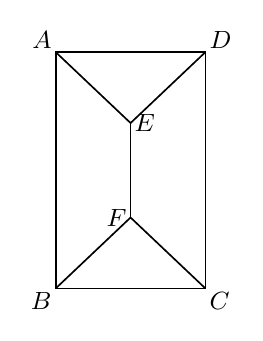
\begin{tikzpicture}[semithick, every node/.style={inner sep=1.2pt, font=\small}]
  \coordinate (A) at (0,3);
  \coordinate (D) at (1.9,3);
  \coordinate (B) at (0,0);
  \coordinate (C) at (1.9,0);
  \coordinate (E) at (0.95,2.1);
  \coordinate (F) at (0.95,0.9);
  \draw (A) -- (D) -- (C) -- (B) -- cycle;
  \draw (A) -- (E) -- (D);
  \draw (B) -- (F) -- (C);
  \draw (E) -- (F);
  \node[above left] at (A) {$A$};
  \node[above right] at (D) {$D$};
  \node[below left] at (B) {$B$};
  \node[below right] at (C) {$C$};
  \node[right] at (E) {$E$};
  \node[left] at (F) {$F$};
\end{tikzpicture}
